\documentclass{article}
\usepackage{titling}
\usepackage{lipsum}
\usepackage{amsmath}
\usepackage{listings}
\usepackage{graphicx}
\usepackage{subcaption}
\usepackage{pgfplots}
\usepackage[margin=1in]{geometry}
\usepgfplotslibrary{statistics}



\begin{document}
\noindent
\begin{minipage}[t]{0.6\textwidth}
    \begin{flushleft}
        \LARGE\textbf{Math 343 - Lab 6} \\
        \vspace{6pt} % add 6pt of vertical space
        \hrule width 10cm
        \vspace{12pt}
        \large\textbf{Preston Duffield} \\
        \large Western Washington University \\
        \today
        % April 18, 2023
        \vspace{24pt}
    \end{flushleft}
\end{minipage}

\section*{Question 1}

\subsection*{a)}

\textbf{Main and interaction effects} \\

\begin{equation*}
\begin{array}{c|c|c}
    \text{Effect} &\text{Coefficient} (\hat{\tau}_1)& \text{Main Effect} (-2\hat{\tau}_1)\\
    \hline
    \text{A} &0.17    & -0.34\\
    \text{B} &5.67    & -11.34\\
    \text{C} &3.42    & -6.84\\
    \text{AB} &-0.83  & 1.66\\
    \text{AC} &-4.42  & 8.84\\
    \text{BC} &-1.42  & 2.84\\
    \text{ABC} &-1.08 & 2.16\\

\end{array}
\end{equation*}\\

\subsection*{b)}

\begin{figure}[h]
    \centering
    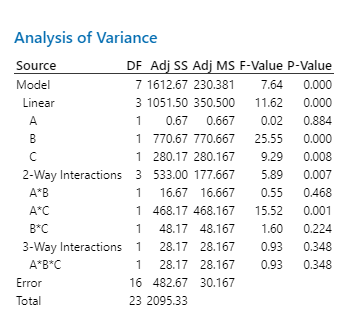
\includegraphics[width=0.5\textwidth]{./images/1_b.png}
    \caption{Anova table from Minitab.}
    \label{fig:3_b_2}
\end{figure}

The following effects are significant (p-value $< \alpha = 0.05$), B, C, AC, and BC.

\subsection*{c)}
\textbf{95\% C.I. For the true main effect of B.} \\
\begin{align*}
    \hat{B} &\pm t_{\alpha/2, df_{error}} \cdot \frac{\sqrt{MSE}}{\sqrt{n \cdot 2^{k-2}}} \\
            &\pm t_{0.025, 16} \cdot \frac{\sqrt{30.167}}{\sqrt{3 \cdot 2^{3-2}}} \\
            &\pm 2.120 \cdot \frac{\sqrt{30.167}}{\sqrt{3 \cdot 2^{3-2}}} \\
            &\pm 4.753640093
\end{align*}
Thus, the confidence interval is $(0.916, 10.423)$
We are 95\% confident that the true main effect of tool geometry (B), is between 0.916 and 10.423.
\subsection*{d)}
\subsection*{e)}
\subsection*{f)}

\clearpage
\section*{Question 2}
First we note that the contrast vectors will have $2^5 = 32$ values.
The last 16 elements of the contrast vectors for A,C,E are as follows
\begin{equation*}
    \vec{A} = \begin{bmatrix}\vdots \\ - \\ + \\ - \\ + \\ - \\ + \\ - \\ + \\ \vdots\end{bmatrix}
    \text{, }
    \vec{C} = \begin{bmatrix}\vdots \\ - \\ - \\ - \\ - \\ + \\ + \\ + \\ + \\ \vdots \end{bmatrix}
    \text{, }
    \vec{E} = \begin{bmatrix}\vdots \\ + \\ + \\ + \\ + \\ + \\ + \\ + \\ + \\ \vdots \end{bmatrix}
\end{equation*}
Note that $\vec{A}$ alternates between $-$ and $+$, every other.
$\vec{C}$ alternates between $-$ and $+$, every 4.
$\vec{E}$ alternates between $-$ and $+$, every 16.

Thus, $\vec{AC} = \vec{A} \times \vec{C}$, is 
\begin{equation*}
    \vec{AC} = \begin{bmatrix}\vdots \\ + \\ - \\ + \\ - \\ - \\ + \\ - \\ + \\ \vdots \end{bmatrix}
\end{equation*}

Finally, the last 16 elements of $\vec{ACE}$ is
\begin{equation*}
    \vec{ACE} = \vec{AC} \times \vec{E} =
    \begin{bmatrix}\vdots \\ + \\ - \\ + \\ - \\ - \\ + \\ - \\ + \\  + \\ - \\ + \\ - \\ - \\ + \\ - \\ + \end{bmatrix} \times \begin{bmatrix}\vdots \\ + \\ + \\ + \\ + \\ + \\ + \\ + \\ + \\ + \\ + \\ + \\ + \\ + \\ + \\ + \\ +  \end{bmatrix}
    = \begin{bmatrix}\vdots \\ + \\ - \\ + \\ - \\ - \\ + \\ - \\ + \\  + \\ - \\ + \\ - \\ - \\ + \\ - \\ + \end{bmatrix}
\end{equation*}

\end{document}
